\chapter*{Preface}
\addcontentsline{toc}{chapter}{Preface}

\sect{VPL and Scratch}

VPL is a visual programming environment for the Thymio robot
(Figure~\ref{fig.vpl}). Scratch (Figure~\ref{fig.scratch}) is a
web-based visual programming environment that animates \emph{sprites} on
the computer screen. The two environments have similar features: a
program is created by dragging-and-dropping blocks onto the screen, and
the fundamental programming construct is the \emph{event handler}.
Therefore, knowledge of one environment can be helpful in learning the
other.

\begin{figure}[hb]
\centering
    \subfigure[VPL]{
		\label{fig.vpl}
		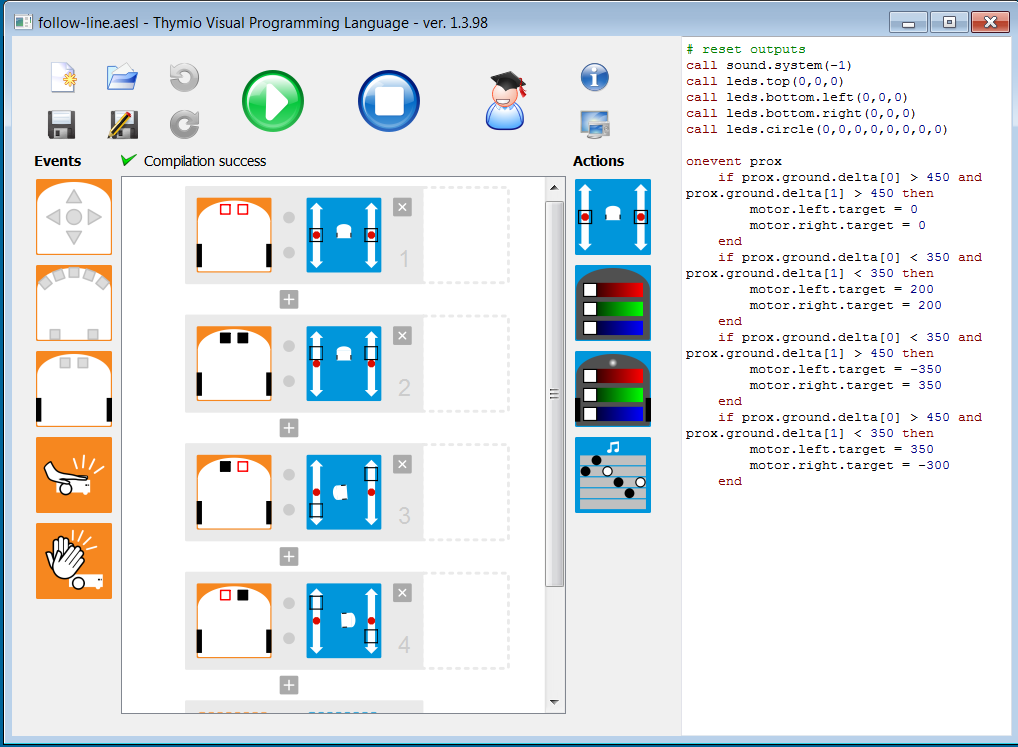
\includegraphics[width = 0.4\textwidth]{gui}
	}
	\hspace{1.5cm}
    \subfigure[Scratch]{
		\label{fig.scratch}
		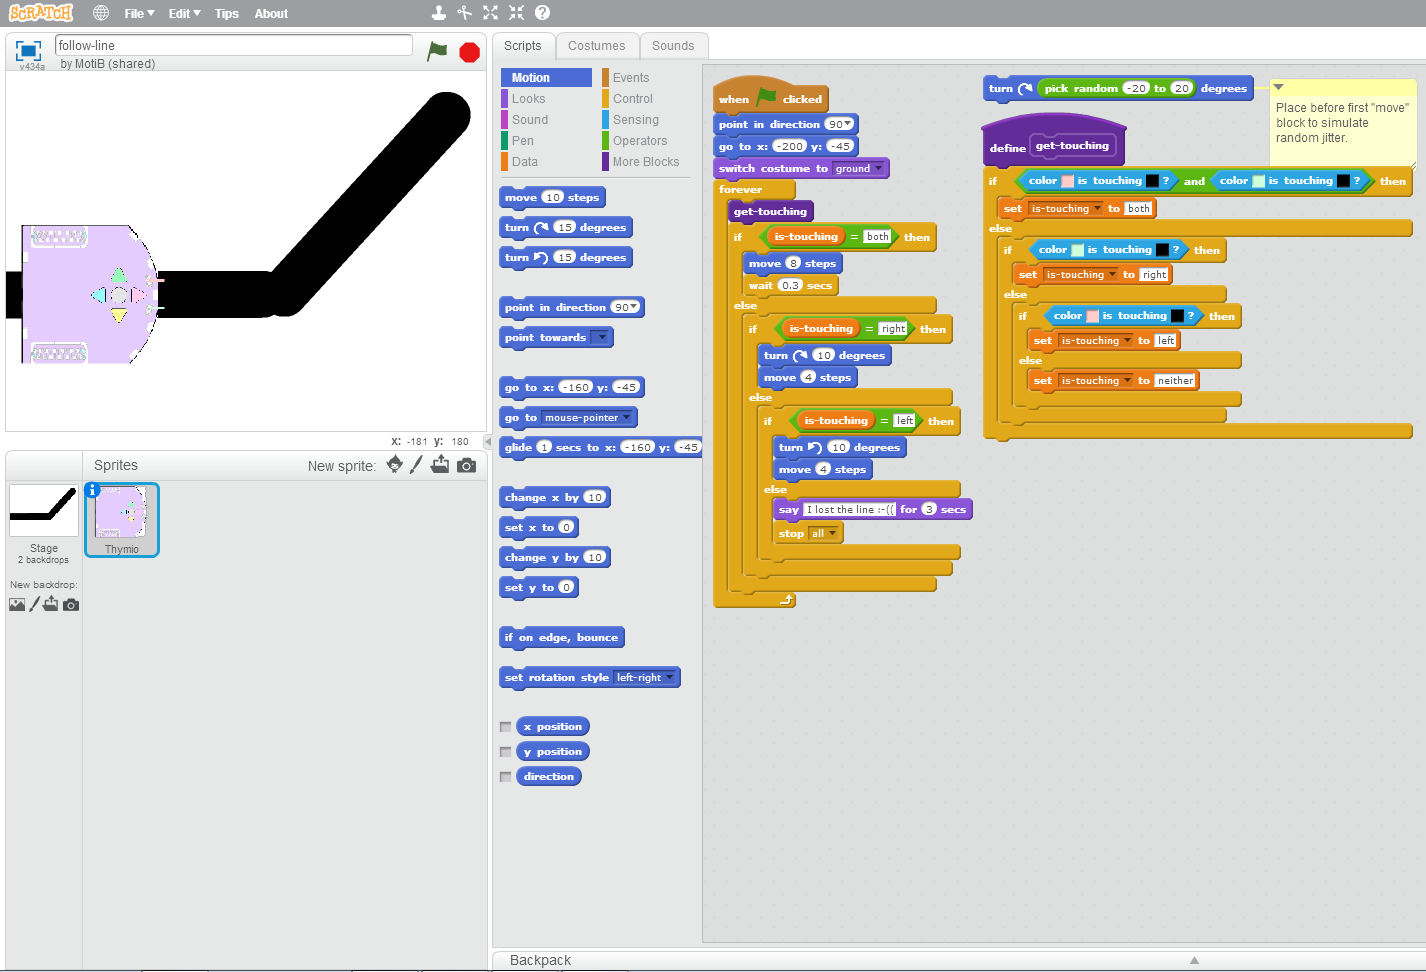
\includegraphics[width = 0.4\textwidth]{scratch}
	}
    \caption{VPL and Scratch}
    \label{fig.vplscratch}
\end{figure}

This document is about transfer from VPL to Scratch. It takes programs
from the VPL tutorial \emph{First Steps in Robotics with the Thymio-II
Robot and the Aseba/VPL Environment}
(\url{https://aseba.wikidot.com/en:thymioprogram}) and shows how to
implement them as Scratch programs controlling a sprite that is an
image of the Thymio robot.

\sect{References}

The document is not intended as a tutorial on Scratch, but
rather as a collection of projects that can be used when learning
Scratch. For an introduction to Scratch, I recommend \textit{Computer
Science Concepts in Scratch} by Michal Armoni and Moti Ben-Ari, which
can be downloaded for free at
\url{http://stwww.weizmann.ac.il/g-cs/scratch/scratch_en.html}.

The projects are arranged in increasing complexity of the Scratch
implementation, not in the order they appear in the VPL tutorial.

The Scratch projects described here can be found in my Thymio studio on
the Scratch website (\url{http://scratch.mit.edu/studios/1023692}). For
other robotics-related Scratch projects, see my website or my Robotics
studio (\url{http://scratch.mit.edu/studios/520857}).

\sect{On the implementation}

Aside from the obvious difference between the concrete Thymio robot and
its image on the Scratch stage, the main difference between the robotic
projects and the Scratch projects is how the sensors are implemented in
Scratch. Full details of the implementation are given in
\cref{ch.implementation}, but it is not necessary to understand them,
since a set of abstractions has been introduced and they will be
described as they are introduced in the projects.

\begin{itemize}

\item A sprite called \p{Pointer} is used to sense where the mouse is
clicked. It broadcasts the messages \p{center}, \p{front}, \p{back},
\p{left}, \p{right} to simulate touching the buttons.

\item The new block \scrblk[-6]{get-pointer-direction-block} returns in the
variable \scrblk[-4]{direction-to-pointer} the direction from the
\p{Thymio} sprite to the point where the mouse was clicked.

\item The new block \scrblk[-6]{get-touching-block} returns in the variable
\scrblk{is-touching} an indication if the \p{left} or \p{right} ground
sensors are touching a black tape, or if \p{both} sensors or \p{neither}
sensor are touching the tape.

\end{itemize}

The following costumes are used:

\begin{itemize}

\item The \p{Thymio} sprite is colored violet to make it stand out on the
stage. You can change this color if you like. The buttons are colored and these
colors should not be changed.

\item Five costumes (\p{blank}, \p{red}, \p{green}, \p{blue},
\p{yellow}) simulate the top lights.

\item The costume \p{ground} simulates the ground sensors.

\end{itemize}
